\noindent
\graphicspath{{./16-08/Images/}} 
%%%%%%%%%%%%%%%%
% Page de gauche
%%%%%%%%%%%%%%%%
\begin{minipage}[t][\textheight][t]{0.33\textwidth}
    \colorbox{StrongBlue}{
        \parbox[c][\textheight][c]{\textwidth}{ 
            \color{OffWhite} 
            \begin{center}
                \noindent
                \begin{minipage}[t][0.55\textheight][c]{0.8\textwidth}
                    {\huge \textbf{Samedi 16 Août}}\\
                    \normalsize
                    \begin{center}
                        \begin{tabular}{@{} l @{\hspace{0.5cm}} l @{}}
                            Abri de départ : &\hfill Vannes \\ 
                            Abri d'arrivée : &\hfill Crouesty \\ 
                            Distance : &\hfill 12 Milles \\ 
                            Départ : &\hfill 11 h 00 \\ 
                            Arrivée prévue : &\hfill 17 h 00 \\ 
                            Lever soleil 
\includegraphics[width=8px,height=8px]{../../Pictos/soleil_OffWhite.png}
 : &\hfill 07 h 09 \\ 
                            Coucher soleil 
\includegraphics[width=8px,height=8px]{../../Pictos/lune_OffWhite.png} : &\hfill 21 h 20 \\ 
                            \\
                            Abris replis : &  \\
                                    & • Arradon \\
                                    & • Île au Moines \\
                                    & • Port Navalo \\                    
                                
                        \end{tabular}
                    \end{center}
                    
                \end{minipage}%

                \begin{minipage}[t][0.4\textheight][t]{\textwidth}

                    \begin{center}
    {\large \textit{Marées \textbf{Port Navalo}}}\\ \vspace{0.5em}
    
    \renewcommand{\arraystretch}{1.40} % Adjust the row height by a factor of 1.4
    
    \begin{tabular}{ |C{5em}|c|C{4em}|C{4em}|}\hline
        & Coef & Heure & Hauteur\\ \hline
        PM & \multirow{2}{1em}{62}      & 10 h 29 & 4,18 m\\ \cline{1-1} \cline{3-4}
        BM &                            & 17 h 08 & 1,50 m\\ \hline
        PM & \multirow{1}{1em}{55}      & 23 h 20 & 4,11 m\\ \hline
    \end{tabular}
\end{center}

                    \begin{center}
    {\large \textit{Marées port de \textbf{Vannes}}}\\ \vspace{0.5em}
    
    \renewcommand{\arraystretch}{1.40} % Adjust the row height by a factor of 1.5
    
    \begin{tabular}{ |C{5em}|c|C{4em}|C{4em}|}\hline
        & Coef & Heure & Hauteur\\ \hline
        BM &\multirow{1}{1em}{68}   & 06 h 26 & 0.48 m\\\hline 
        PM &\multirow{2}{1em}{62}   & 12 h 35 & 2,63 m\\ \cline{1-1} \cline{3-4}
        BM &                        & 18 h 53 & 0,53 m\\\hline 
    \end{tabular}
\end{center}
                \end{minipage}%
            \end{center}       
        }      
    }
\end{minipage}%
\begin{minipage}[c][\textheight][t]{0.10\textwidth}
\hfill
\end{minipage}%
\begin{minipage}[c][\textheight][t]{0.50\textwidth}
    \vspace{4cm}
    \color{StrongBlue}    
    {\huge \textbf{Description de la navigation}}\\
            \begin{itemize}
                \item Départ de Vannes à 11 h après prise en main des bateaux par les équipages. Remontée du chenal au moteur pour hissage des voiles une fois Roguedas passée. Si le vent est portant un gênois seul peut être déployé pour remonter plus rapidemment le chenal. 
                \item Rappel et pratique des manoeuvres de base entre Roguedas et les Logodens (virements + empannages).
                \item Prise de coffre à Arradon et repas vers 12 h 30. 
                \item Départ vers 13 h 30, passage nord Logodens direction la Jument. Points d'attention au passage de la Truie, puis aux Réchauds qu'on laissera largement sur bâbord. 
                \item Top à la manoeuvre sur le banc de Kergonan. Arrivée à la jument prévue un peu avant 16 h 00 pour passer avec la fin du jusant.
                \item Arrivée au Crouesty vers 17 h 00.
                \item C'est la première journée de navigation du camp, on ne manquera pas de s'assurer de l'état des troupes à l'arrivée. 
            \end{itemize}
        {
        \huge \textbf{Contraintes de la navigation}}\\
            \begin{itemize}
                \item Le pont de Vannes qui sera ouvert entre 10h30 et 14h30. 
                \item Passage de la jument avant 17h pour éviter la marée montante. Idéalement après 15h30 pour éviter le moment ou la marée est la plus forte.  
                \item En fonction des conditions de vent, il est envisageable de passer la jument à la voile. On allumera quand même le moteur au point mort en sécurité et on hésitera pas à enrouler le gênois et à finir en route moteur si le passage s'avère plus difficile que prévu. 
            \end{itemize}
\end{minipage}%
%%%%%%%%%%%%%%%%
% Page de droite
%%%%%%%%%%%%%%%%
\newgeometry{top=2cm, bottom=2cm, left=2cm, right=2cm}
\begin{minipage}[t][0.9\textheight][t]{0.60\textwidth}
    \color{StrongBlue}    
    \noindent
    \begin{minipage}[t][0.3\textheight][t]{\textwidth}
        \begin{minipage}[t][0.3\textheight][t]{0.65\textwidth}
            \vspace{-8.5em}
            {\huge \textbf{Détails de la navigation}}\\
            Le QR-code situé à droite est cliquable, il permet d'explorer le planning de navigation sur le site datashom. 
            La carte ci-dessous visualise le trajet prévu ainsi que les abris de replis et dangers identifiés. 
        \end{minipage}%
        \hfill
        \begin{minipage}[t][0.3\textheight][t]{0.25\textwidth}       
        \href{https://data.shom.fr/datacontext/fr/1730379753617-147640}{ 
            
\includegraphics[width=0.8\textwidth]{qr-code.png}
        }
        \end{minipage}%
    \end{minipage}
    \begin{minipage}[t][0.7\textheight][t]{\textwidth}
        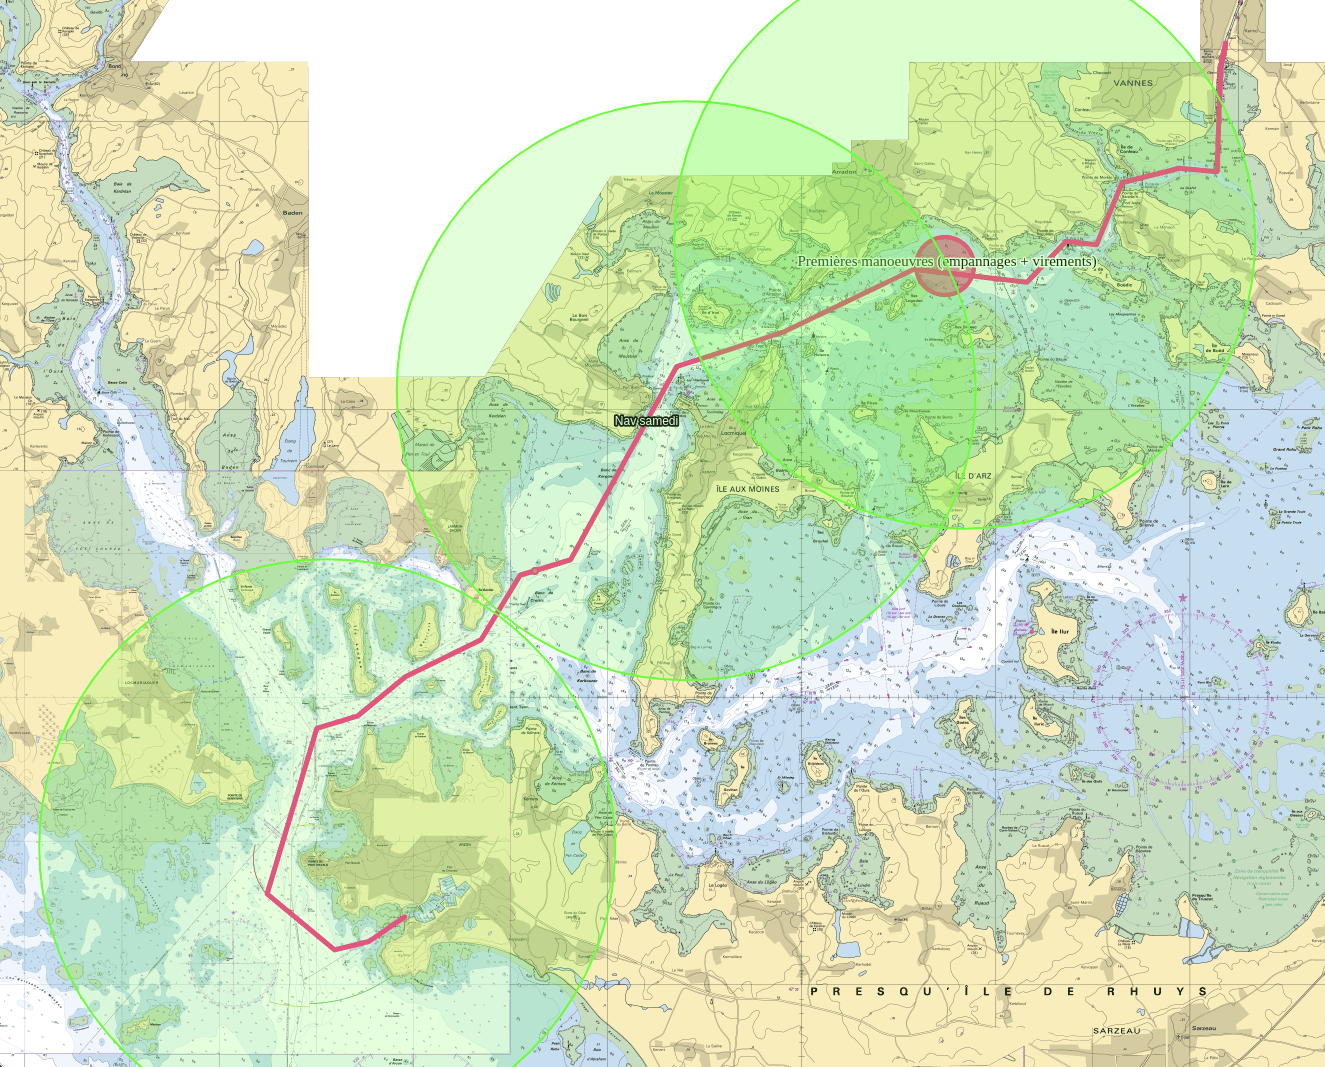
\includegraphics[height=0.7\textheight]{carte.png}
    \end{minipage}
\end{minipage}
\begin{minipage}[t][0.9\textheight][t]{0.40\textwidth}
    \color{StrongBlue} 
    \centering 
    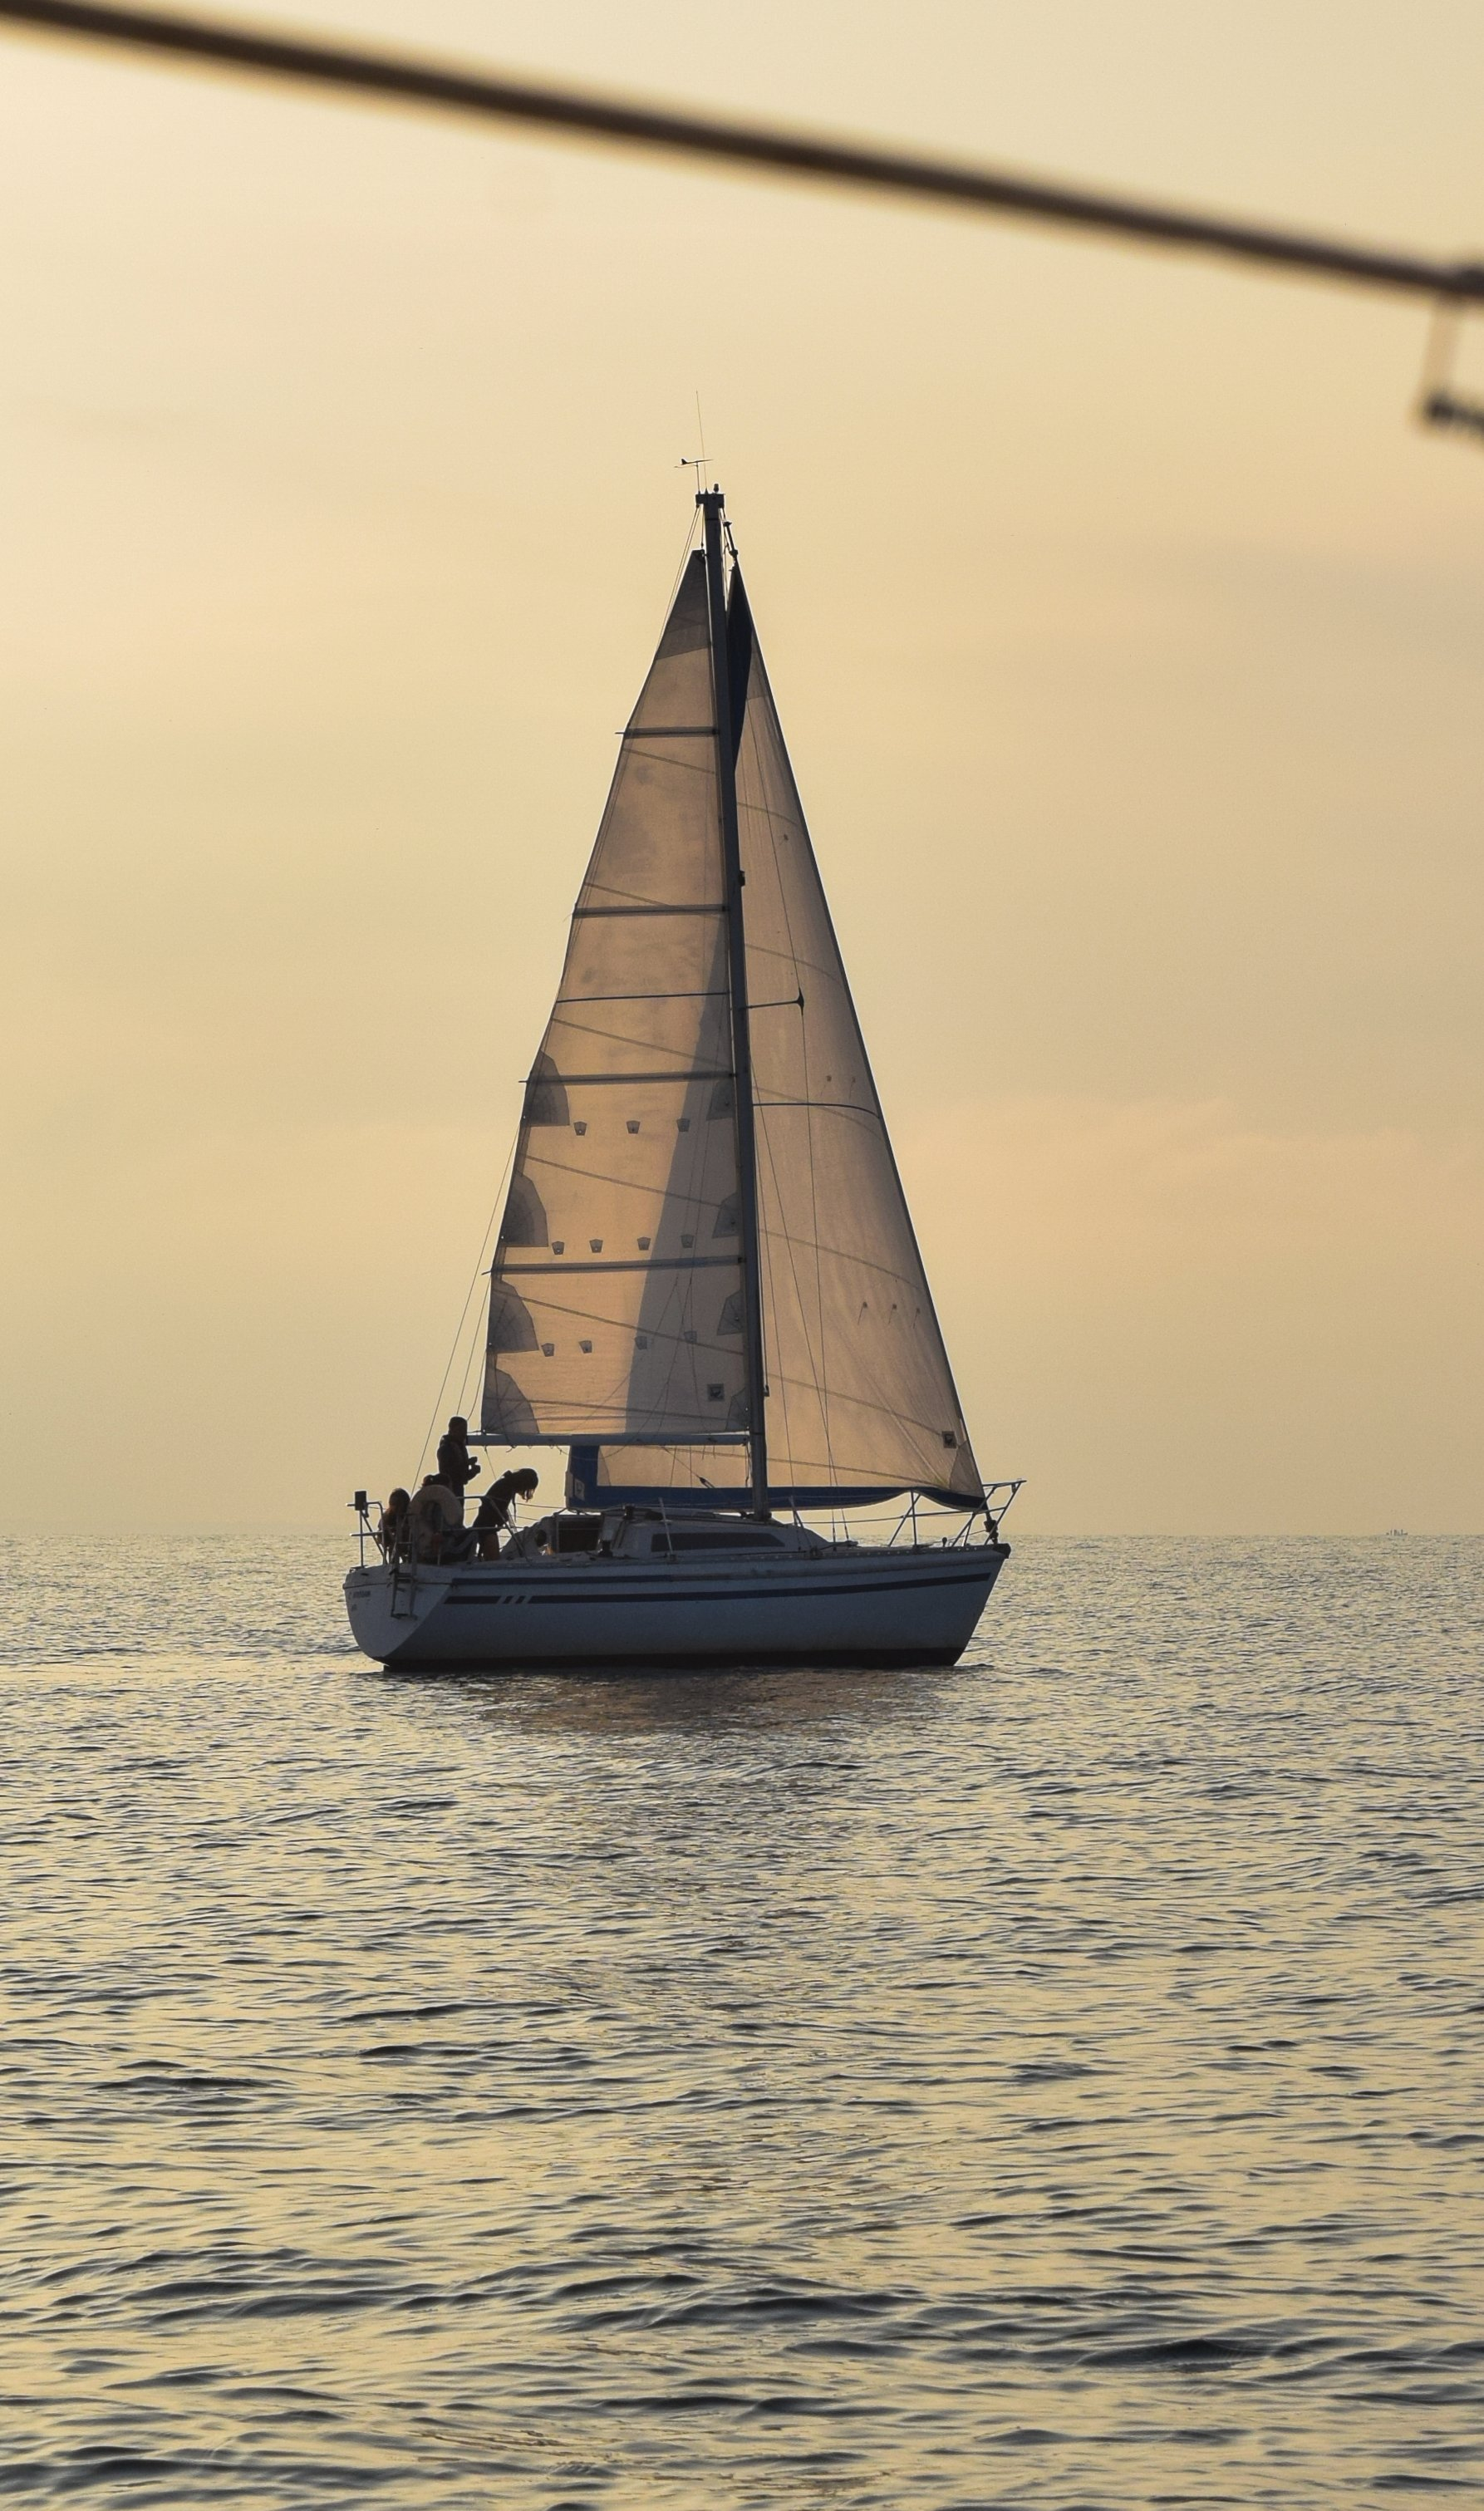
\includegraphics[height=\textheight, width=\textwidth, keepaspectratio]{illustration_verticale.jpg}
\end{minipage}%
\restoregeometry



